\documentclass{article}
\usepackage[utf8]{inputenc}
\usepackage[english]{babel}
\usepackage[a4paper, total={7in, 9in}]{geometry}
\usepackage{graphicx}
\usepackage{float}
\usepackage{verbatim}
\usepackage{fancyvrb}
\usepackage[bottom]{footmisc}
\PassOptionsToPackage{hyphens}{url}\usepackage{hyperref}
\usepackage[style=numeric]{biblatex}
\usepackage{csquotes}
\usepackage[title]{appendix}
\usepackage{xcolor}
\usepackage{minted}

\addbibresource{references.bib}

\newcommand{\question}[1]{
    {\large \textbf{Q: #1}}
    \\
}

\newcommand{\titleRule}{
    \rule{\linewidth}{0.5mm} \\ [0.25cm]
}

\begin{document}

{
\center
\textsc{\Large Universidade do Minho} \\ [0.5cm]
\textsc{\Large Masters in Computer Engineering} \\ [0.5cm]
\textsc{\large Parallel Algorithms} \\ [0.5cm]

{\LARGE \bfseries Parallel Gauss-Seidel method} \\[0.2cm]
{\LARGE \bfseries for solving the heat transfer problem} \\[0.5cm]

\begin{tabular}{c c}
    José Carlos Lima Martins & Miguel Miranda Quaresma \\
    A78821 & A77049  \\
\end{tabular} \\[0.5cm]

\today \\[1cm]
}

\section{Introduction}

The heat transfer problem, in a two dimensional space (2D), deals with determining how the temperature at each point of a surface evolves over time
until a steady state is reached, at which point the temperature remains constant (equilibrium temperature). 
Each point starts at a certain temperature which changes due to the action of heat sources located at the boundaries of the plane, that cause heat to
disperse across the surface.

\subsection{Problem Modelling}
The heat transfer problem, as previously mentioned, deals with the diffusion of heat in a surface over time until it reaches a steady state (equilibrium). 
In a 2 dimensional plane, with coordinates $(x,y)$, the problem can be modeled by the \textbf{heat equation} as follows:

$$\frac{\partial u}{\partial t} = \frac{\partial^2u}{\partial x^2} + \frac{\partial^2u}{\partial y^2}$$

which represents the variation of temperature ($u(x,y)$) at a certain point.

Since the objective is to determine the temperature of each point when steady state is reached \textbf{i.e.} when heat transfer no longer 
occurs ($=0$), the problem can be described by the following equation:

$$\frac{\partial u}{\partial t} = 0 \Rightarrow \frac{\partial^2u}{\partial x^2} + \frac{\partial^2u}{\partial y^2} = 0$$

A caveat of the steady-state equation is that it doesn't imply that every point on the plane is at the same temperature, allowing for temperature gradients to be 
present in the plate. However, given the heat sources remain constant, the temperature gradients will remain constant after steady state is reached.

To determine the temperature at any given point in a plate it's then necessary to apply the presented equation to each point of the plate. One obvious way of 
doing this is using a system of linear equations where each line is the steady state temperature at a point.

Taking the previous equation we can now determine the temperature at a certain point when steady state is reached using the following expression:

$$\frac{\partial^2u}{\partial x^2} + \frac{\partial^2u}{\partial y^2} \\
\Rightarrow \frac{u(x+h/2, y) + u(x-h/2, y) - 2u(x,y)}{h^2} + \frac{u(x, y+k/2) + u(x, y-k/2) - 2u(x,y)}{k^2}$$

To calculate the temperature difference between two points, different steps, $h$ and $k$, can be used for each of the coordinates $x$ and $y$, leading to an error
of magnitude $O(h^2)$ and $O(k^2)$ respectively.


\subsection{Approach}
The use of iterative methods to solve computational problems is motivated by the need to solve large scale problems such as systems of linear equations with
a considerable number of variables. In this cases, the use of a direct method, while providing an exact solution, would require a considerable
amount of computing power and time to execute, making iterative methods more suitable for such scenarios. One example of such method is the 
Gauss-Seidel iterative method that works by continuously updating a matrix containing the coefficients of each equation in each line where each element is 
updated as follows:

$$x_i^{k+1} = \frac{b_i - \sum_{j=1}^{i-1} a_{ij}x_j^{k+1} - \sum_{j=i+1}^n a_{ij}x_j^k}{a_{ii}}$$

where $k$ is the current iteration. \\
The method halts when the differences between iterations are under a predefined threshold/tolerance. 
This improves on the Jacobi method by using the values of the elements that have already been computed to update the current element, resulting in a higher 
convergence rate as well dispensing the need for storing two vectors as only the most recent values are needed. However, by using the most recent 
values, this method introduces data dependencies in each iteration, making it harder to develop in a parallel paradigm (as we will see in a later section, 
this can be overcome by applying a strategy known as Red-Black strategy).

Another important factor to take into consideration when solving large scale problems is the use of matrix-free methods. Such approaches don't require
the (coefficient) matrix to be explicitly stored in memory, as that would require a large amount of memory and computing time, accessing the coefficients
by using matrix-vector products. 
However, for the sake of simplicity, the implementations developed in the present work use a matrix to store the coefficients of each equation in each 
line of the matrix.

\subsection{Discretization}
Calculating the temperature at every point in a 2D plane in a continuous domain would be infeasible as it would require an infinite amount of points.
As such, it becomes necessary to transfer the domain from a continuous one to a discrete one through a process known as discretization.
This process works by applying a mesh to the continuous domain and taking the value of the function (being studied) at each point of the mesh. In the case of the heat
equation the mesh is composed of four boundaries, called heat sources, with known temperature values, and a set of internal points whose temperature
is unknown. The process of discretization introduces a truncation error due to the fact that less points than the initial problem are used to describe the 2D
plane. As such, the truncation error is inversely proportional to the amount of points in the mesh. 

\begin{figure}[H]
    \centering
    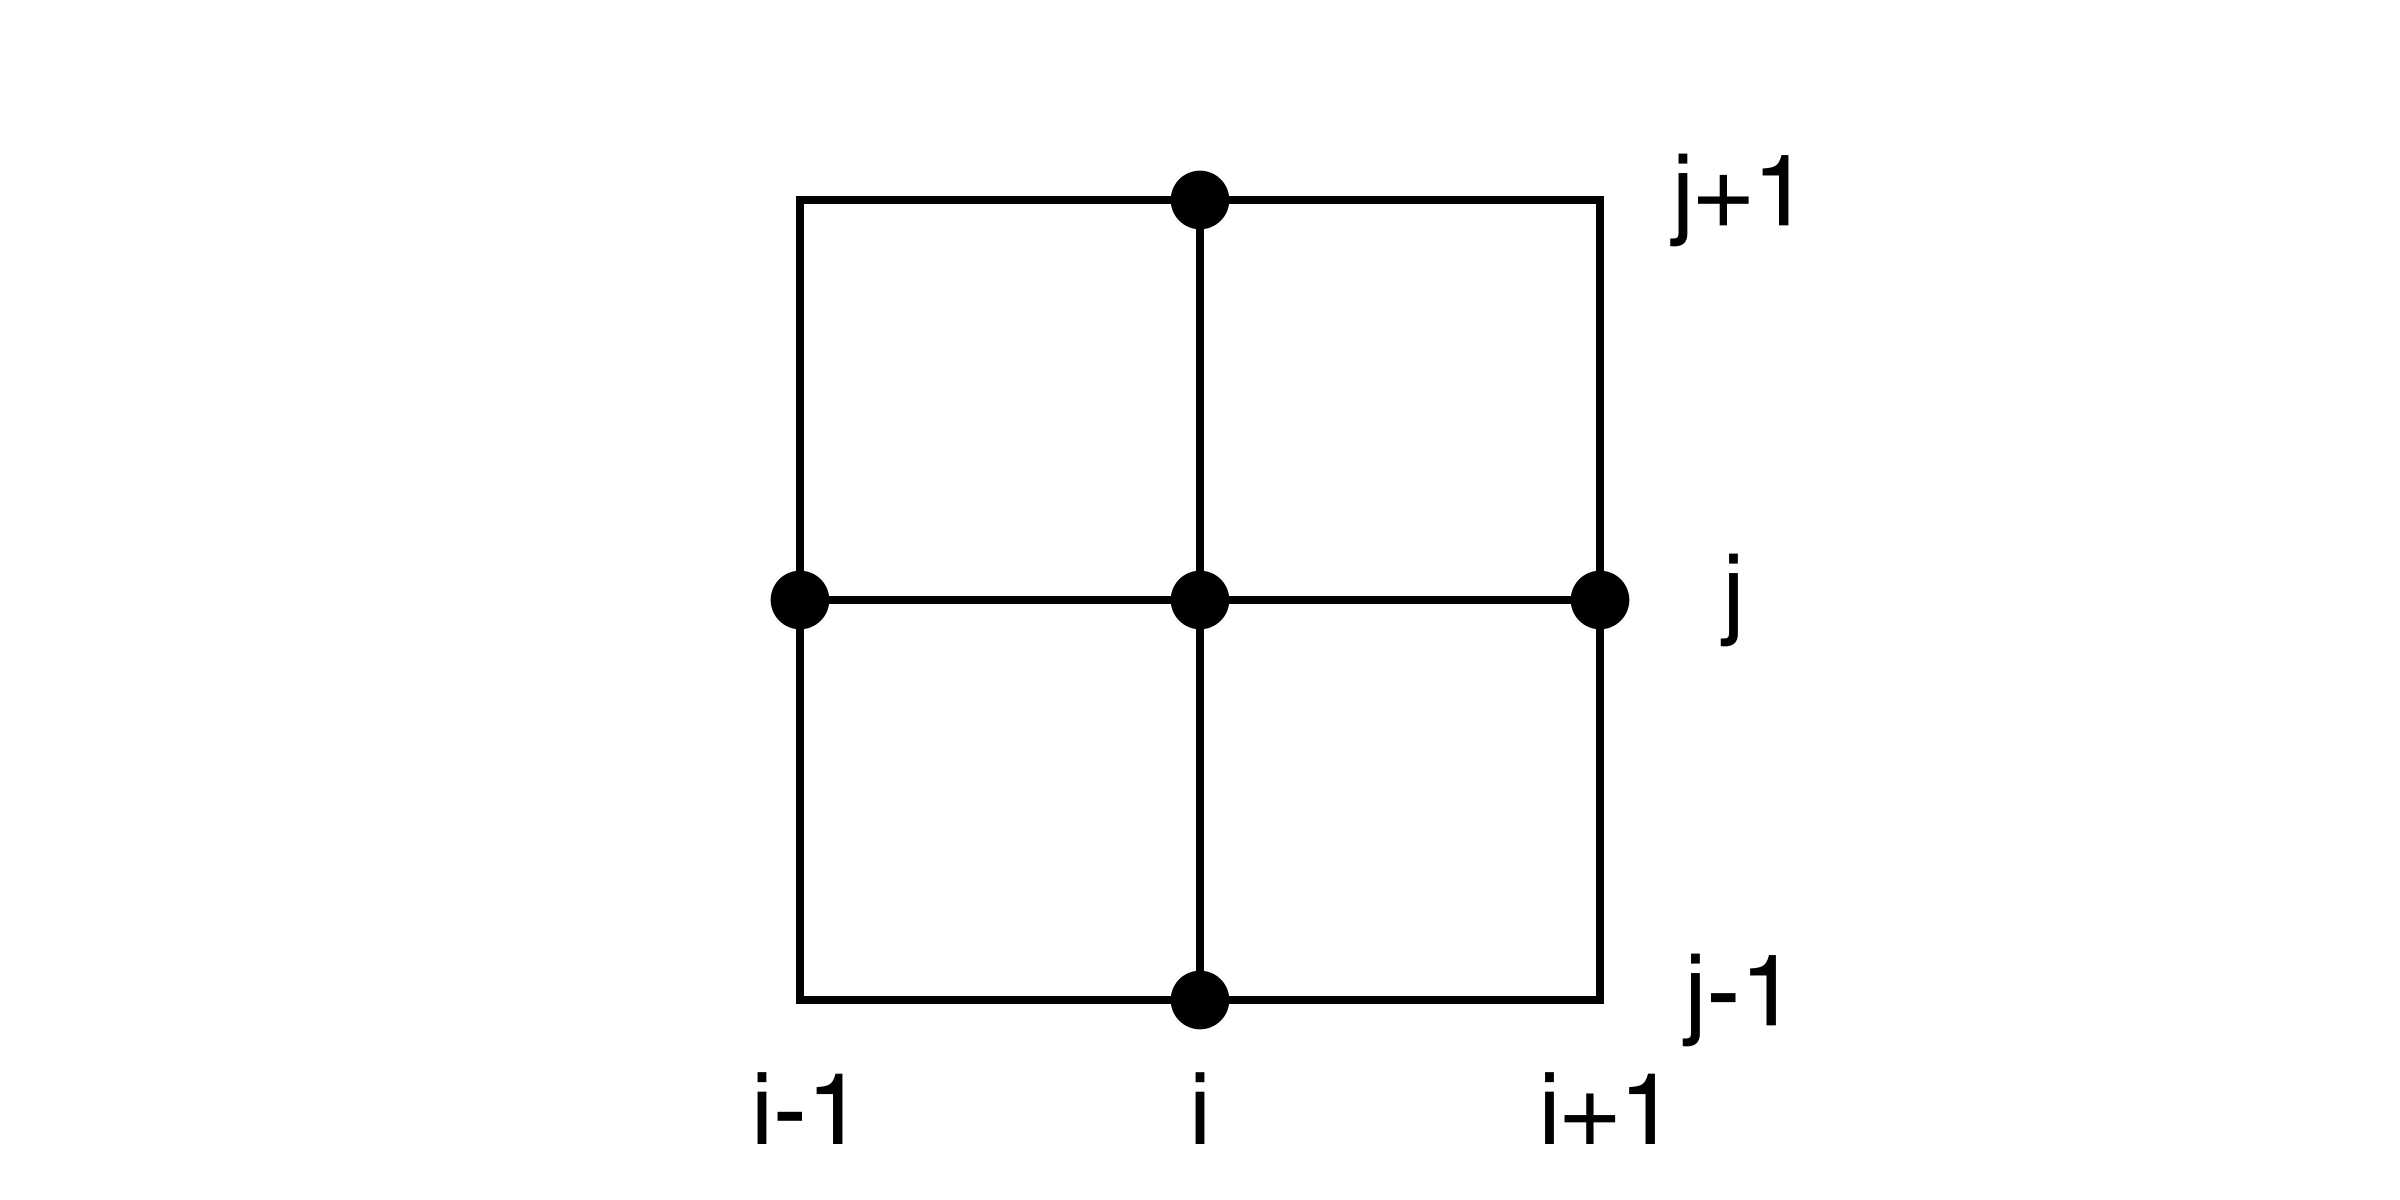
\includegraphics[width=10cm]{Pictures/Discretization.png}
    \caption{Discretization on a 2D plane with a five-point stencil}
    \label{fig:discretization}
\end{figure}

This truncation error in a mathematical perspective it's a swap of partial derivatives for stencils (approximation), i.e. use of finite differences. As such, 
each point will be updated according to a five-point stencil, using the the arithmetic average of the four neighbouring points and the central point as the 
new value. In other words, with a centered finite differences approach the truncation error will be $O(h^2)$ where $h$ is the distance between two 
consecutive points in the mesh ($h=1$ when using Gauss-Seidel).


\section{Benchmark Platform}
In order to better understand the benchmark results gathered a brief description of the conditions in which the benchmarks were
executed will be presented.

\subsection{Statistical Methods}
A sample size of one was used for each benchmark because the number of iterations required don't change between different executions 
of the same benchmark.

\subsection{Hardware Platform}
The benchmarks hereby mentioned were executed on a cluster node, from the SeARCH Computing Infrastructure. The node used, r641,
presents the following hardware specifications~\cite{cpu,search}:
\begin{itemize}
    \item \textbf{CPU}: Intel Xeon E5-2650v2 @2.6GHz, 16 cores
    \item \textbf{Cache Size}:
    \begin{itemize}
        \item L1d (per core): 32 KiB
        \item L1i (per core): 32 KiB
        \item L2 (per core): 256 KiB
        \item L3 (per package): 20 MiB
    \end{itemize}
    \item \textbf{RAM}: 64GB
    \item \textbf{Network}: Ethernet, \textit{myrinet}
\end{itemize}

\section{Sequential Implementation}
When implementing problems such as the heat transfer problem that deal with large quantities of data, and operations per 
element/unit of data, it's important to consider an approach that allows for easy parallelization. However, in order to better understand the 
problem being solved, a sequential implementation of the problem was developed initially, from which the pseudo-parallel (or parallel-ready)
implementation was based off.

The sequential implementation (see \ref{seqImp}) begins by defining a tri-dimensional matrix made up of two \texttt{N} by \texttt{N} matrices 
that store the temperature values of the plate at each iteration. It begins by initializing the top, left and right boundaries of the plate 
at 100 and the bottom one with 0 while the internal points are initialized with a value of 50. 
Based on the size of the plate \textbf{i.e.} number of points in the mesh(N), a tolerance is set for the difference between temperatures
in consecutive iterations.
The function \texttt{poissongs} implements the Gauss-Seidel method on the matrix and halts the loop when the stopping criteria is met:
$$|| u^{k+1} - u^k|| \leq TOL$$
At each iteration, the last temperature values are stored in the matrix indexed as \texttt{plate[last]}.
Additionally, the biggest difference between consecutive temperatures in a point, is stored in \texttt{dif} which is used to check whether
the stopping criteria has been met. 

\section{Sequential Implementation with Red-Black Strategy}
Based on the sequential implementation, a parallel-ready implementation was developed (see \ref{seqRBImp}) using the Red-Black strategy for dealing 
with data dependencies in each iteration. This strategy works by interleaving the updated points in each loop so that it's possible for
the loop load to be distributed amongst different processes without needing to deal with data dependencies. It achieves this by updating the matrix in two
different loops, one for updating the odd points(Red) and the other for updating the even points(Black). Even though there are no dependencies in
each of the loops, the order at which the loops are executed must be preserved (Red-Black). A \textit{caveat} to this mechanism is the fact that the Red 
points stencil uses the old values for temperature: 
$$x_i^{k+1} = \frac{b_i - \sum_{j=1}^n a_{ij}x_j^k}{a_{ii}}$$
while the Black points stencil uses the current temperature values of it's neighboring elements: 
$$x_i^{k+1} = \frac{b_i - \sum_{j=1}^n a_{ij}x_j^{k+1}}{a_{ii}}$$
This property results in a bigger number of iterations needed as the method tends to converge at a slower rate. The stop criteria is the same as 
the previously stated.

\section{Parallel Implementation (MPI) with Red-Black Strategy}
The development of parallel applications is usually divided into two different paradigms the shared memory paradigm and the distributed memory paradigm.
The choice between the two is influenced not only by the characteristics of the work load, but also by the intended result. The development of 
parallel applications using a distributed memory paradigm via libraries such as OpenMPI allows for a thorough theoretical analysis of the expected
behaviour of the algorithm, which is useful for identifying possible bottlenecks before developing the application. 
The parallel implementation developed uses OpenMPI and distributes the load between each process. Due to the characteristics of OpenMPI, this (initial) 
distribution doesn't require a broadcast of any values to each process as their memory is copied from the parent process, which contains the matrix with the
initial temperatures for each point in the mesh. The load distribution process begins by calculating the number of lines assigned to each process, which 
is given by the expression: $\frac{N-2}{number\_processes}$  where $N$ is the number of lines. The process with rank $P-1$ is assigned with the remaining 
lines \textbf{i.e.} $ (N-2) \bmod P$:

\begin{figure}[H]
    \centering
    \includegraphics[width=10cm]{Pictures/MatrixDraw.png}
    \caption{Load distribution}
    \label{fig:lineDiv}
\end{figure}

Each process then invokes the \texttt{phase} function which updates a group of rows of the mesh based on the process rank. To ensure the order at which
the mesh points are updated complies with the Red-Black scheme, the function \texttt{updateValues} is called after updating the Red points, and each process
exchanges one line with the two neighbouring processes (rank-1 and rank+1):

\begin{figure}[H]
    \centering
    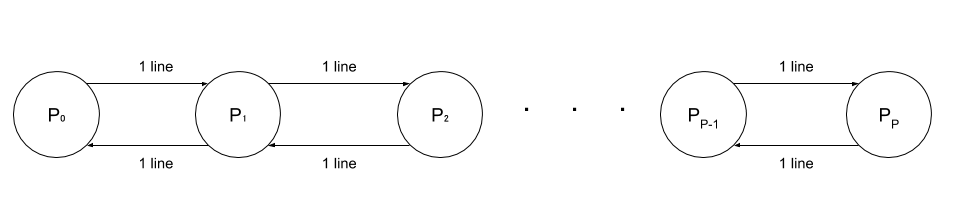
\includegraphics[width=13cm]{Pictures/IterationCommunication.png}
    \caption{Function \texttt{updateValues}}
    \label{fig:commuLines}
\end{figure}

At the end of each iteration, the function \texttt{updateValues} is invoked again and every process communicates the biggest difference 
between two consecutive temperatures for a given point to the parent process (with rank 0), which then determines the biggest value
between all this differences. This value is then communicated back to each process which use it to check whether the method has reached an 
acceptable solution. After all iterations are executed, it is necessary to collect (communicate) the data from all the processes, which 
is gathered by the parent process. 

\begin{figure}[H]
    \centering
    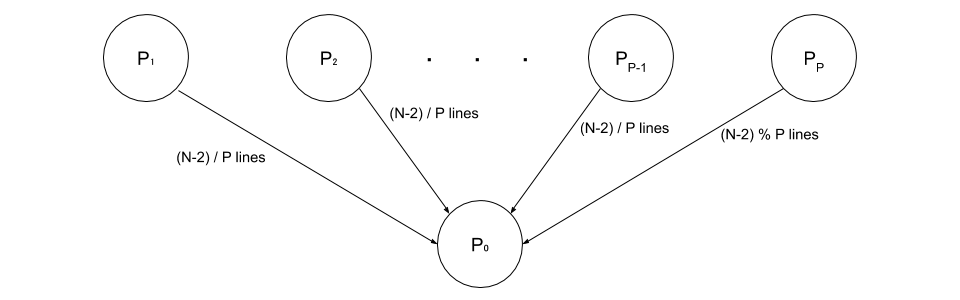
\includegraphics[width=13cm]{Pictures/FinalCommunication.png}
    \caption{Result gathering}
    \label{fig:commuLines}
\end{figure}

The total amount of data exchanged between processes can be estimated as a function of the mesh size $N$, the number of processes $P$ 
and the number of iterations $it$ by the following expression:

$$ it * ( 2*2N*(P-1) + 2(P-1) ) + \frac{N-2}{P}*N*(P-1)$$

where:

\begin{itemize}
    \item $2*2N*(P-1)$ corresponds to the amount of data transferred in each iteration
    \item $2(P-1)$ corresponds to the amount of data needed to determine the biggest difference between two consecutive temperature values
    \item $\frac{N-2}{P}*N*(P-1)$ corresponds to the amount of data gathered after all iterations are executed
\end{itemize}

From this expression it's obvious that the amount of data transferred is of order $O(N^2)$ based on the mesh size.

\newpage

\section{Analysis and comparison of the different approaches}

To understand the behaviour of each implementation, and more specifically, how the Red-Black strategy affects the number of iterations needed
to obtain an acceptable solution, each implementation was run with 3 different parameters for the mesh size (10, 100, 1000) as well as different
tolerance values: $TOL=\frac{1}{N^2}$. The following chart shows the number of iterations needed, for each implementation, to reach an acceptable 
solution based on this parameters: 

\begin{figure}[H]
    \centering
    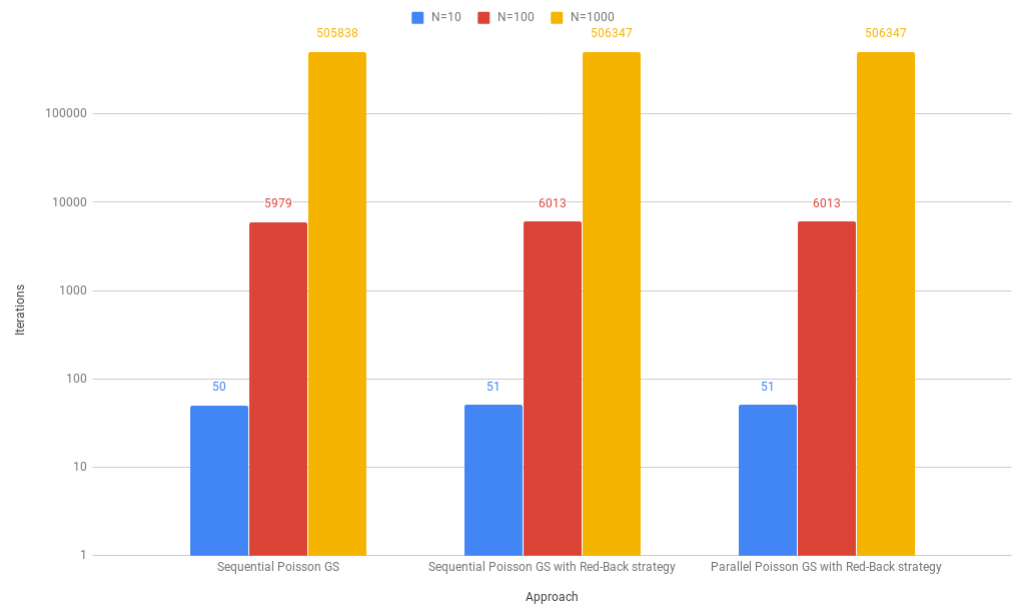
\includegraphics[width=16cm]{Pictures/Results.png}
    \caption{Results}
    \label{fig:results}
\end{figure}

One noticeable aspect of the results is the fact that the Red-Black strategy requires a higher number of iterations to obtain an acceptable solution,
which comes as a consequence of the fact that the Red points are updated using old values for it's neighbouring points which are then used by the Black
points, resulting in a slower convergence rate. Additionally, an increment on the size of the mesh, $N$, leads to a higher number of iterations until
the stop criteria is met. This is to be expected as the tolerance value is a function of the mesh size, becoming more restrictive as this value increases. 
Thus, the convergence rate is lower for bigger $N$ values, while the the cost of each iteration increases since there are more elements to be updated.
The number of iterations increases proportional to a logarithmic scale. 
Finally, the use of a parallel version via MPI, which distributes the load between more than one process (Parallel with RB), while requiring the same number
of iterations as it's sequential counterpart (Sequential with RB), will result in a reduced execution time.

\section{Conclusion}
The experiments on this work show that the usage of strategy such as Red-Black, in conjunction with an iterative method such as Gauss-Seidel, for solving 
the heat dispersion problem is indeed advantageous for dealing with data dependencies that would, otherwise, make parallelization infeasible.
This remains true even with an increase in the number of iterations needed to reach an acceptable solution as the workload distribution outweighs
this increase when it comes to performance and execution time.
Additionally, the use of an iterative method such as Guass-Seidel, allows for an acceptable solution to be obtained for linear systems that would 
otherwise take a considerable amount of execution time and computing power to solve.

\printbibliography

\newpage 
\begin{appendices}

\section{Code}

\subsection{Auxiliar Code (utils)}
\begin{framed}
\begin{minted}{c}
#include "utils.h"

/**
 * Initialize heat plate with temperature values
 */
void initPlate(float plate[][N][N]){
    for(int i = 0; i < N; i ++){
        plate[0][0][i] = 100.0f;
        plate[0][i][0] = 100.0f;
        plate[0][i][N-1] = 100.0f;
        plate[0][N-1][i] = 0.0f;

        plate[1][0][i] = 100.0f;
        plate[1][i][0] = 100.0f;
        plate[1][i][N-1] = 100.0f;
        plate[1][N-1][i] = 0.0f;
    }

    for(int i = 1; i < N-1; i ++)
        for(int j = 1; j < N-1; j ++)
            plate[0][i][j] = 50.0f;

    plate[0][N-1][0] = 0.0f;
    plate[1][N-1][0] = 0.0f;
}

void initPlateForMPI(float plate[][N*N]){
    for(int i = 0; i < N; i ++){
        plate[0][0*N+i] = 100.0f;
        plate[0][i*N+0] = 100.0f;
        plate[0][i*N+N-1] = 100.0f;
        plate[0][(N-1)*N+i] = 0.0f;

        plate[1][0*N+i] = 100.0f;
        plate[1][i*N+0] = 100.0f;
        plate[1][i*N+N-1] = 100.0f;
        plate[1][(N-1)*N+i] = 0.0f;
    }

    for(int i = 1; i < N-1; i ++)
        for(int j = 1; j < N-1; j ++){
            plate[0][i*N+j] = 50.0f;
            plate[1][i*N+j] = 50.0f;
        }

    plate[0][(N-1)*N+0] = 0.0f;
    plate[1][(N-1)*N+0] = 0.0f;
}
\end{minted}
\end{framed}

\subsection{Sequential Implementation}\label{seqImp}
\begin{framed}
\begin{minted}{c}
#include "utils.h"

/*
 * Returns the number of iterations performed
 */
int poissongs(float plate[][N][N], float tol){
    int it = 0, last=0;
    float dif = tol + 1.0f, temp;

    while(dif > tol){
        dif = 0.0f;             //differences at the borders are 0.0f
        for(int i = 1; i < N-1; i ++)
            for(int j = 1; j < N-1; j ++){
                plate[!last][i][j] = (plate[!last][i-1][j] + plate[!last][i][j-1] 
                                    + plate[last][i][j+1] + plate[last][i+1][j]) / 4.0f;
                temp = fabs(plate[!last][i][j] - plate[last][i][j]);
                if(temp > dif) dif = temp;
            }
        it ++;
        last = !last; //update matrix
    }
    return it;
}


int main(int argc, char *argv[]){
    float plate[2][N][N];
    float tol = 1.0f / (N*N);
    int it;

    initPlate(plate);

    it = poissongs(plate, tol);
    printf("Sequential Poisson GS\n Iteration Count: %d\n", it);

    return 0;
}
\end{minted}
\end{framed}

\subsection{Sequential Implementation with Red-Black Strategy}\label{seqRBImp}
\begin{framed}
\begin{minted}{c}
#include "utils.h"

/*
 * Returns the number of iterations performed
 */
int poissongs(float plate[][N][N], float tol){
    int it = 0, last=0;
    float dif = tol + 1.0f, temp;

    while(dif > tol){
        dif = 0.0f;             //differences at the borders are 0.0f
        //Black
        for(int i = 1; i < N-1; i ++)
            for(int j = 2 - i%2; j < N-1; j +=2){
                plate[!last][i][j] = (plate[last][i-1][j] + plate[last][i][j-1] 
                                    + plate[last][i][j+1] + plate[last][i+1][j]) / 4.0f;
                temp = fabs(plate[!last][i][j] - plate[last][i][j]);
                if(temp > dif) dif = temp;
            }

        //Red
        for(int i = 1; i < N-1; i ++)
            for(int j = 1 + i%2; j < N-1; j +=2){
                plate[!last][i][j] = (plate[!last][i-1][j] + plate[!last][i][j-1] 
                                    + plate[!last][i][j+1] + plate[!last][i+1][j]) / 4.0f;
                temp = fabs(plate[!last][i][j] - plate[last][i][j]);
                if(temp > dif) dif = temp;
            }

        it ++;
        last = !last; //update matrix
    }
    
    return it;
}


int main(int argc, char *argv[]){
    float plate[2][N][N];
    float tol = 1.0f / (N*N);
    int it;

    initPlate(plate);

    it = poissongs(plate, tol);

    printf("Sequential Poisson GS with Red-Back strategy\n Iteration Count: %d\n", it);

    return 0;
}
\end{minted}
\end{framed}

\subsection{Parallel Implementation (MPI) with Red-Black Strategy}\label{parRBImp}
\begin{framed}
\begin{minted}[fontsize=\footnotesize]{c}
#include <mpi.h>
#include "utils.h"

void updateValues(float plate[][N*N], int last, int offset, int rows, int rank, int no_procs, MPI_Status status){
    if(!rank){
        MPI_Recv( &(plate[last][(rows+1)*N]), N, MPI_FLOAT, rank+1, 2, MPI_COMM_WORLD, &status );
        MPI_Send( &(plate[last][rows*N]), N, MPI_FLOAT, rank+1, 2, MPI_COMM_WORLD);
    }else{
        MPI_Send( &(plate[last][(offset+1)*N]), N, MPI_FLOAT, rank-1, 2, MPI_COMM_WORLD);

        if(rank!=no_procs-1)
            MPI_Recv( &(plate[last][offset*N + (rows+1)*N]), N, MPI_FLOAT, rank+1, 2, MPI_COMM_WORLD, &status );

        if(rank!=no_procs-1)
            MPI_Send( &(plate[last][offset*N + rows*N]), N, MPI_FLOAT, rank+1, 2, MPI_COMM_WORLD);

        MPI_Recv( &(plate[last][offset*N]), N, MPI_FLOAT, rank-1, 2, MPI_COMM_WORLD, &status );
    }
}

float phase(float plate[][N*N], int last, int offset, int rows, int rank, int no_procs, MPI_Status status){
    float dif, temp;
    dif = 0.0f;

    //Black
    for(int i = offset+1; i < offset + 1 + rows; i ++)
        for(int j = 2 - i%2; j < N-1; j +=2){
            plate[!last][i*N+j] = (plate[last][(i-1)*N+j] + plate[last][i*N+j-1] 
                                + plate[last][i*N+j+1] + plate[last][(i+1)*N+j]) / 4.0f;
            temp = fabs(plate[!last][i*N+j] - plate[last][i*N+j]);
            if(temp > dif) dif = temp;
        }

    updateValues(plate, !last, offset, rows, rank, no_procs, status);

    //Red
    for(int i = offset+1; i < offset + 1 + rows; i ++)
        for(int j = 1 + i%2; j < N-1; j +=2){
            plate[!last][i*N+j] = (plate[!last][(i-1)*N+j] + plate[!last][i*N+j-1] 
                                + plate[!last][i*N+j+1] + plate[!last][(i+1)*N+j]) / 4.0f;
            temp = fabs(plate[!last][i*N+j] - plate[last][i*N+j]);
            if(temp > dif) dif = temp;
        }

    updateValues(plate, !last, offset, rows, rank, no_procs, status);

    if(rank){
        MPI_Send( &dif, 1, MPI_FLOAT, 0, 1, MPI_COMM_WORLD);
        MPI_Recv( &dif, 1, MPI_FLOAT, 0, 1, MPI_COMM_WORLD, &status);
    }else{
        for(int i=1; i<no_procs; i++){
            MPI_Recv( &temp, 1, MPI_FLOAT, i, 1, MPI_COMM_WORLD, &status);
            if(temp > dif) dif = temp;
        }
        for(int i=1; i<no_procs; i++){
            MPI_Send( &dif, 1, MPI_FLOAT, i, 1, MPI_COMM_WORLD);
        }
    }
    return dif;
}

/*
 * Returns the number of iterations performed
 */
int poissongs(float plate[][N*N], float tol, int rank, int no_procs, MPI_Status status){
    int it = 0, last=0, rows_per_proc, remaining_rows, work_load = N-2, begin, offset;
    float dif = tol + 1.0f;

    rows_per_proc = work_load/(no_procs-1);      //truncates result
    remaining_rows = work_load % (no_procs-1);   //remaining rows

    offset = rank * rows_per_proc;

    while(dif > tol){
        if(rank==no_procs-1)
            dif = phase(plate, last, offset, remaining_rows, rank, no_procs, status);
        else
            dif = phase(plate, last, offset, rows_per_proc, rank, no_procs, status);

        it ++;
        last = !last; //update matrix
    }

    //collect data
    if(!rank){
        begin = (rows_per_proc+1)*N;

        for(int i=1; i<no_procs-1; i++, begin+=rows_per_proc*N)
            MPI_Recv(&(plate[last][begin]), rows_per_proc*N, MPI_FLOAT, i, 3, MPI_COMM_WORLD, &status);

        MPI_Recv(&(plate[last][begin]), remaining_rows*N, MPI_FLOAT, no_procs-1, 3, MPI_COMM_WORLD, &status);

        //copy of process 0 result
        for(int i=1; i<rows_per_proc+1; i++)
            for(int j=0; j<N; j++)
                plate[last][i*N+j]=plate[!last][i*N+j];

    }else if(rank == no_procs-1) {
        MPI_Send( &(plate[!last][(offset+1)*N]), remaining_rows*N, MPI_FLOAT, 0, 3, MPI_COMM_WORLD);
    }else{
        MPI_Send( &(plate[!last][(offset+1)*N]), rows_per_proc*N, MPI_FLOAT, 0, 3, MPI_COMM_WORLD);
    }
    
    return it;
}


int main(int argc, char *argv[]){
    float plate[2][N*N];
    float tol = 1.0f / (N*N);
    int it, rank, no_procs;

    initPlateForMPI(plate);

    //Move MPI process creation to poissongs
    MPI_Status status;
    MPI_Init(&argc, &argv);
    MPI_Comm_size(MPI_COMM_WORLD, &no_procs);
    MPI_Comm_rank( MPI_COMM_WORLD, &rank );

    it = poissongs(plate, tol, rank, no_procs, status);

    MPI_Finalize();

    if(rank == 0)
        printf("Parallel Poisson GS with Red-Back strategy\n Iteration Count: %d\n", it);

    return 0;
}
\end{minted}
\end{framed}

\end{appendices}

\end{document}